\subsection{Bayesian Statistical Inference}
For Bayesian statistics, we have only one formula: Bayes’s rule: 
\[
  \underbrace{f_{\Theta \vert X} (\theta \vert x)}_{\text{posterior}} \propto \underbrace{f_{X \vert \Theta} (x \vert \theta)}_{\text{likelihood}} \underbrace{f_{\Theta} (\theta)}_{\text{prior}}
\]

We have some prior knowledge, and after observing something, we can use the prior (assumption) and likelihood to update our belief, which gives us the posterior. This posterior can later serve as the prior for another observation, allowing us to continuously update our belief throughout the observation process.

\begin{eg}
  Romeo is waiting for Juliet on their first date. He wants to estimate how long he will have to wait for her. Given that Romeo has some prior dating experience, he already has some prior knowledge about how late girls tend to be.
  
  Girl A - \(X \sim \text{Uniform}(0, 0.3)\); 
  
  Girl B - \(X \sim \text{Uniform}(0, 0.8)\); 

  Girl C - \(X \sim \text{Uniform}(0, 0.6)\), 

  where the uniform random variable shows the range of lateness. For example, for girl A, she will be late between the dating time and the dating time plus 0.3 hours. Then, how could you use Bayesian statistics to estimate the waiting time for Romeo's new girlfriend? 

  \textbf{Solution:} 
  Here we can set up the uniform random variable \(\text{Uniform}(0, \Theta)\), where \(\Theta\) depends on the girls. Then what we need to find is the \(\theta\) for Juliet. We can then have 
  \[
    f_{X \vert \Theta}(x \vert \theta) = \begin{dcases}
      \frac{1}{\theta}, &\text{ if } 0 \leq x \leq \theta ;\\
      0, &\text{ otherwise} .
    \end{dcases}
  \]

  In Romeo's model, \(\theta\) is also a uniform random variable \(\theta \sim \text{Uniform}(0, 1)\), where \(X \sim \text{Uniform}(0, \Theta)\). It means that Romeo has a prior belief that all the girls would be late for at most 1 hour, and the likelihood of Juliet being late is described by \(X\), which states that she could be \(\theta\) hour late. Given that on their first date, Juliet arrived \(\frac{1}{2}\) hours late, we have 
  \[
    f_{\Theta \vert X} (\theta \vert \dfrac{1}{2}) \propto f_\Theta (\theta) f_{X \vert \Theta}(\dfrac{1}{2} \vert \theta) = \dfrac{1}{\theta}
  \]
  Here we have the prior \(f_\Theta(\theta) = 1\) if \(0 \leq \theta \leq 1\), and the likelihood \(f_{X \vert \Theta} (\frac{1}{2} \vert \theta) = \frac{1}{\theta}\) if \(\frac{1}{2} \leq \theta \leq 1\). Keep in mind that the prior comes from Romeo's model, where he has never dated a girl who is late for more than 1 hour, and it may not be valid if \(\theta > 1\), which shows the limitation of Bayesian statistics. Also, the observation (likelihood) shows the probability of Juliet arriving precisely at (or within a very small interval around) time plus 0.5. Therefore, we have \(\theta \geq \frac{1}{2}\). Otherwise, if \(\theta < \frac{1}{2}\), it is not possible for Juliet to arrive \(\frac{1}{2}\) hour late, since it is not included in Romeo's belief. 

  For the integral to be equal to 1, we need to find the constant term. This can be found using calculus: 
  \[
    \int_\frac{1}{2} ^1 \dfrac{1}{\theta} d \theta= \ln \theta \Big|_{\frac{1}{2}}^1 = \ln 2 \Longrightarrow f_{\Theta \vert X} (\theta \vert \dfrac{1}{2}) = \dfrac{1}{\theta \ln 2}
  \]

  \begin{minipage}{0.5\textwidth}
    Here we have \(\theta < \frac{1}{2} = 0\) because from the data, we know that \(\theta \geq \frac{1}{2}\), which means the lateness parameter is at least \(\frac{1}{2}\), so it is not possible for Juliet to arrive between the dating time and dating time plus 0.5. We also have \(\theta > 1 = 0\) because from Romeo's prior knowledge, he knows that a girl would not be later than 1 hour.
  \end{minipage}
  \begin{minipage}{0.5\textwidth}
    \centering
    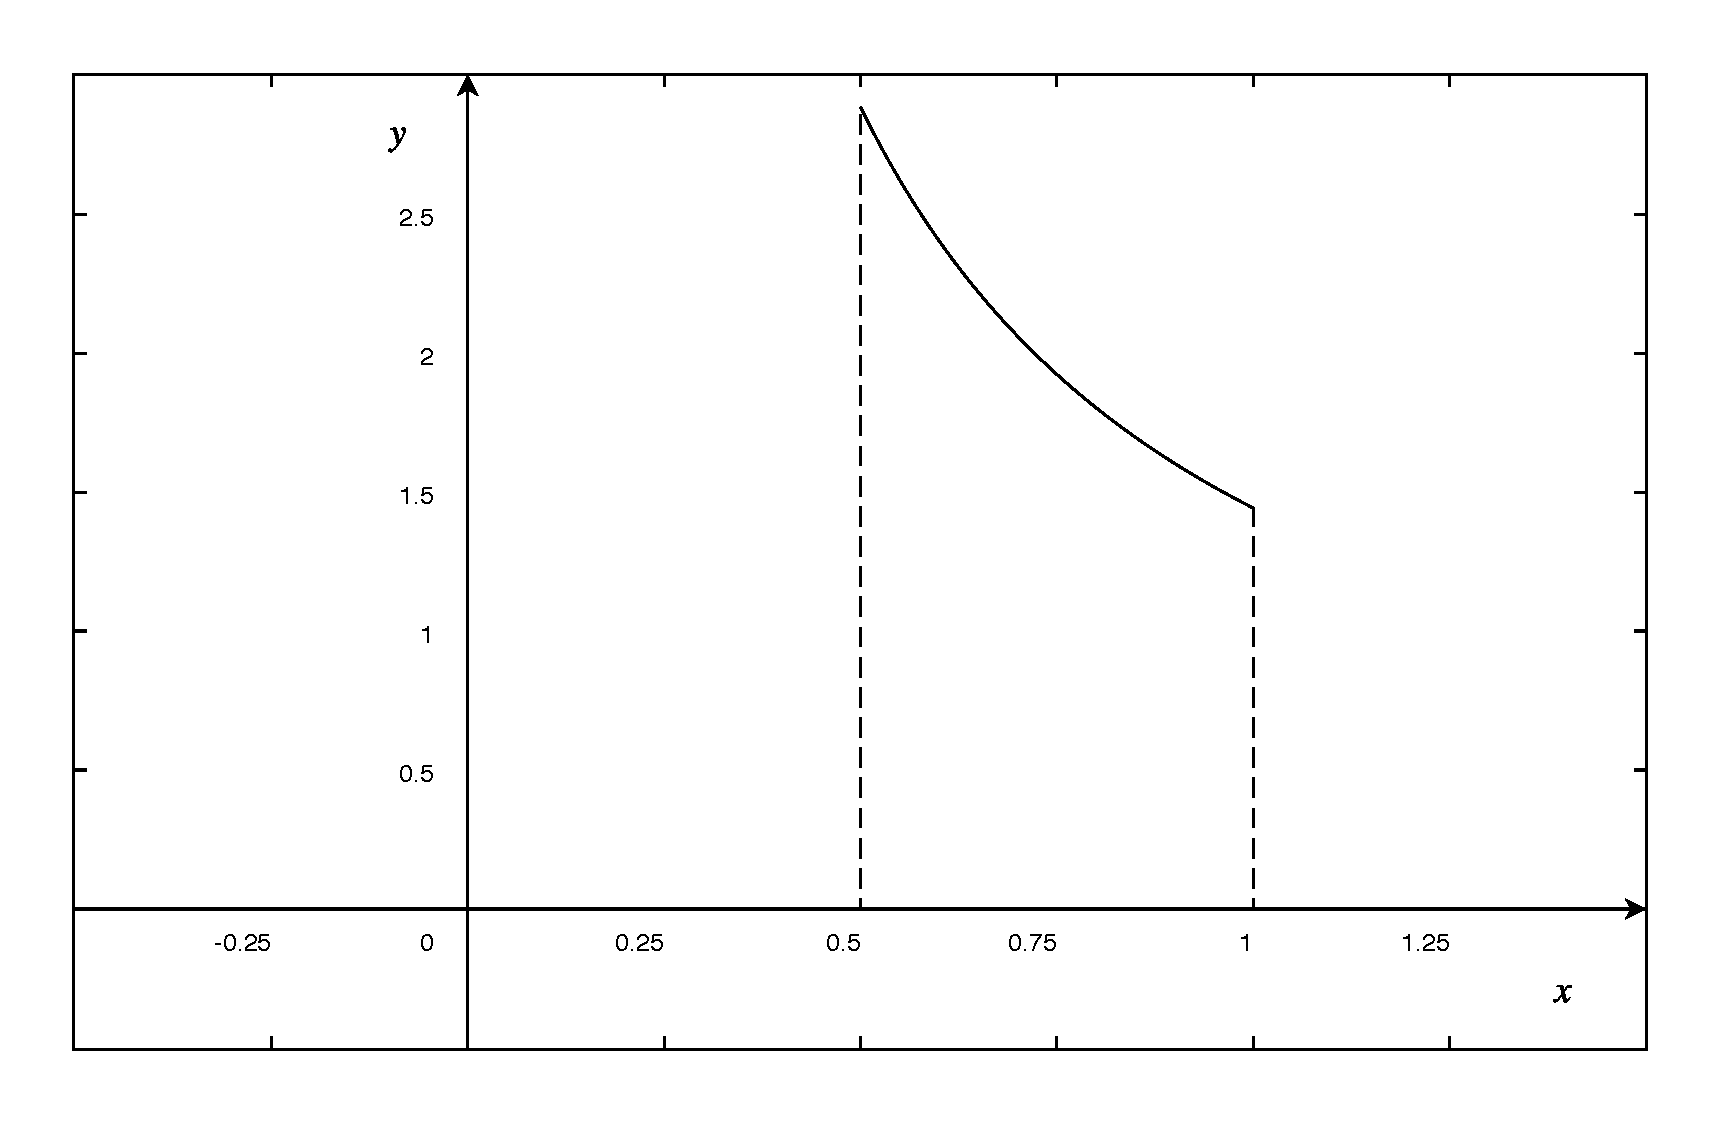
\includegraphics[width=0.8\textwidth]{Figures/Romeo_model.pdf}
  \end{minipage}

  On their second date, Juliet arrived \(\frac{1}{4}\) hours late. We then need to readjust the prior based on the previous model to find the new posterior.
  \[
    f_{\Theta \vert X_1, X_2} \left(\theta \Big| \dfrac{1}{2}, \dfrac{1}{4}\right) \propto f_{\Theta \vert X_1} \left(\theta \Big| \dfrac{1}{2}\right) f_{X_2 \vert \Theta, X_1}\left(\dfrac{1}{4} \Big| \theta, \frac{1}{2}\right)
  \]
  Here, since \(X_1\) and \(X_2\) are independent, we can discard \(X_1\) in the calculation.
  \[
    f_{\Theta \vert X_1, X_2} \left(\theta \Big| \dfrac{1}{2}, \dfrac{1}{4}\right) \propto f_{\Theta \vert X_1} \left(\theta \Big| \dfrac{1}{2}\right) f_{X_2 \vert \Theta}\left(\dfrac{1}{4} \Big| \theta\right) = \dfrac{1}{\theta \ln 2} \times \dfrac{1}{\theta} = \dfrac{1}{\theta^{2} \ln{(2)}} \propto \dfrac{1}{\theta^2}
  \]
  The same as above, we have \(f_{X_2 \vert \Theta} (\frac{1}{4} \vert \theta) = \frac{1}{\theta}\) for \(\theta \geq \frac{1}{4}\) since it is not possible for the lateness to be less than \(\frac{1}{4}\) hours. Also, given the prior as calculated in the first part, we have \(f_{\Theta \vert X_1} (\theta \vert \frac{1}{2}) = \frac{1}{\theta \ln 2}\) if \(\frac{1}{2} \leq \theta \leq 1\).

  For the integral to be equal to 1, we need to find the constant term. This can be found using calculus: 
  \[
    \int_\frac{1}{2} ^1 \dfrac{1}{\theta^2} d \theta = 1 \Longrightarrow f_{\Theta \vert X_1, X_2} \left(\theta \Big| \dfrac{1}{2}, \dfrac{1}{4}\right) = \dfrac{1}{\theta^2}
  \]

  \begin{figure}[H]
    \centering
    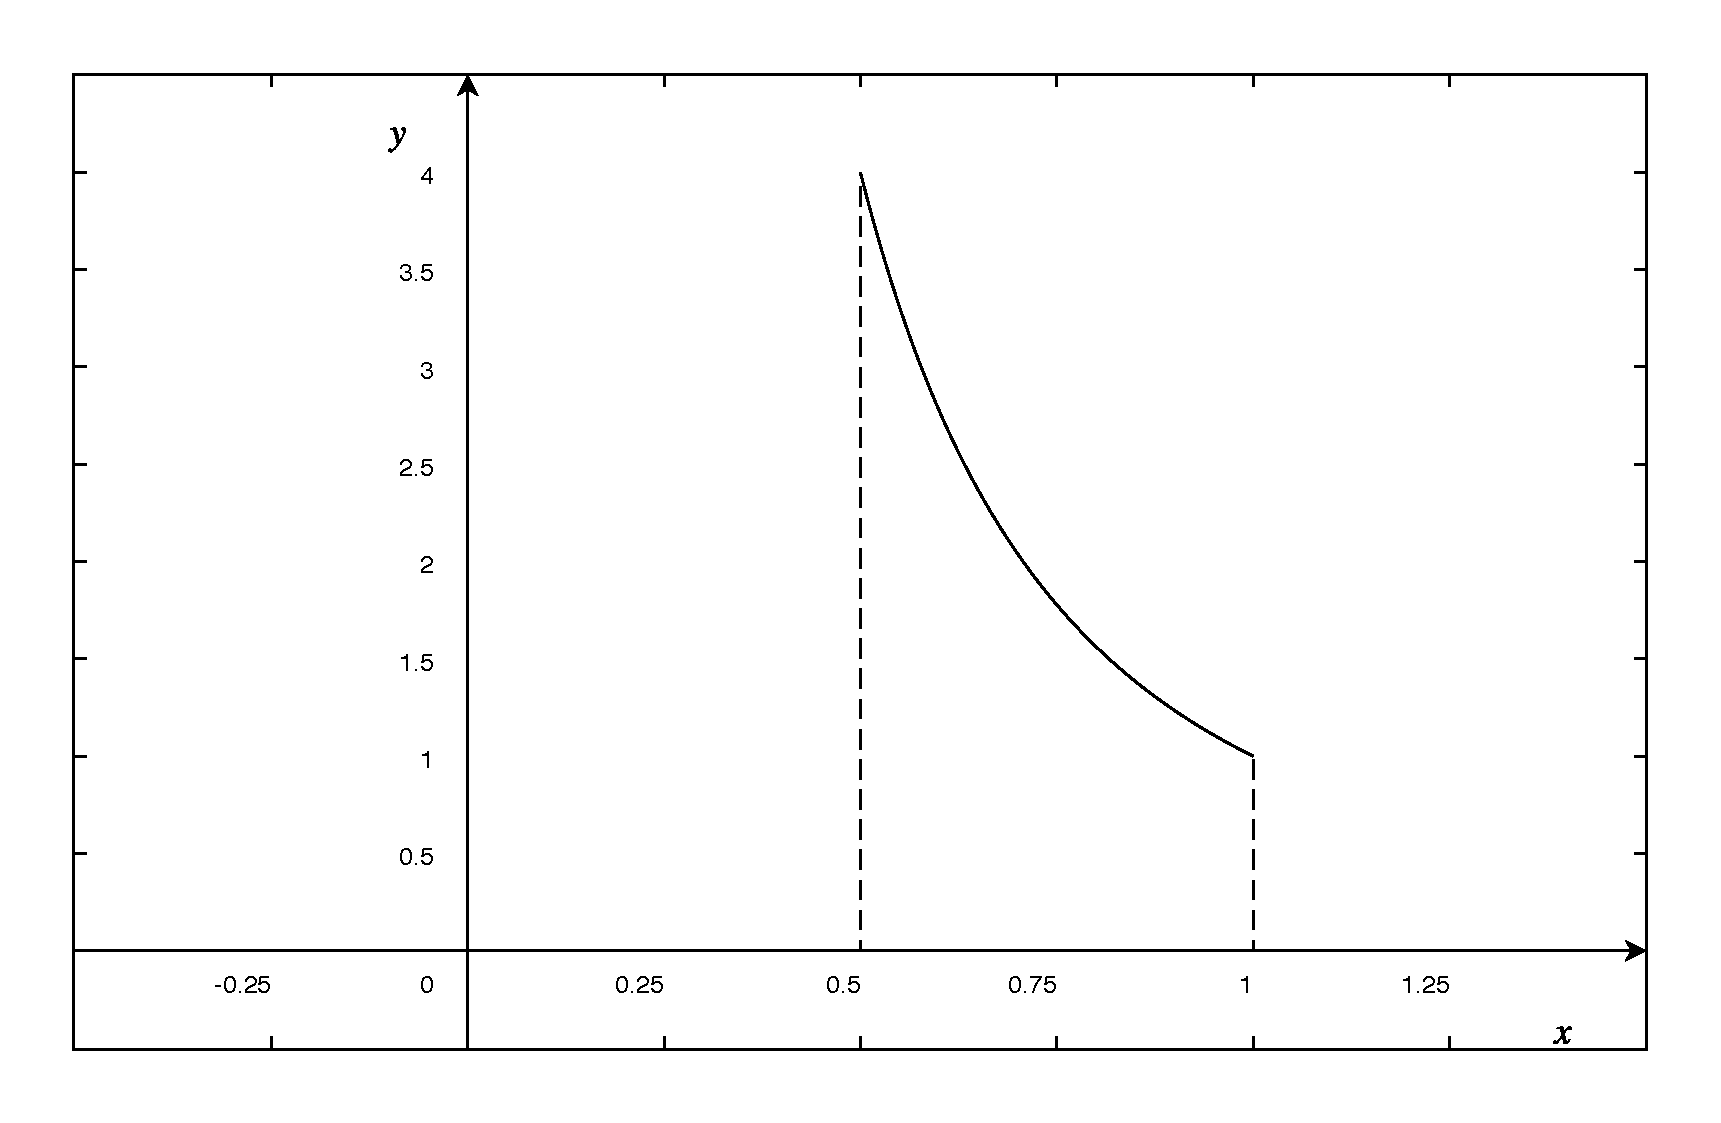
\includegraphics[width=0.5\textwidth]{Figures/Romeo_model_2.pdf}
  \end{figure}
\end{eg}
\begin{remark}[Bayes' rule variant]
  \[
    \mathbb{P}(\theta \vert x_1, x_2) = \dfrac{\mathbb{P}(x_2 \vert \theta, x_1) \mathbb{P}(\theta \vert x_1)}{\mathbb{P}(x_2 \vert x_1)}
  \]
\end{remark}
\begin{proof}
  \[
    \begin{aligned}
      f_{\Theta \vert X_1, X_2} \left(\theta \Big| \dfrac{1}{2}, \dfrac{1}{4}\right) &= \dfrac{f_{\Theta, X_1, X_2} \left(\theta, \dfrac{1}{2}, \dfrac{1}{4}\right)}{f_{X_1, X_2}\left(\dfrac{1}{2}, \dfrac{1}{4}\right)} \\
      &= \dfrac{f_{X_2 \vert \Theta, X_1} \left(\dfrac{1}{4} \Big| \theta, \dfrac{1}{2}\right) f_{\Theta, X_1}\left(\theta, \dfrac{1}{2}\right)}{f_{X_1, X_2}\left(\dfrac{1}{2}, \dfrac{1}{4}\right)} \\
      &= \dfrac{f_{X_2 \vert \Theta, X_1} \left(\dfrac{1}{4} \Big| \theta, \dfrac{1}{2}\right) f_{\Theta \vert X_1}\left(\theta \Big| \dfrac{1}{2}\right) f_{X_1} \left(\dfrac{1}{2}\right)}{f_{X_1, X_2}\left(\dfrac{1}{2}, \dfrac{1}{4}\right)} \\
      &= \dfrac{f_{X_2 \vert \Theta, X_1} \left(\dfrac{1}{4} \Big| \theta, \dfrac{1}{2}\right) f_{\Theta \vert X_1}\left(\theta \Big| \dfrac{1}{2}\right)}{f_{X_2 \vert X_1}\left(\dfrac{1}{4} \Big| \dfrac{1}{2}\right)} \\
    \end{aligned}
  \]
  Thus, 
  \[
    f_{\Theta \vert X_1, X_2} \left(\theta \Big| \dfrac{1}{2}, \dfrac{1}{4}\right) \propto f_{X_2 \vert \Theta, X_1} \left(\dfrac{1}{4} \Big| \theta, \dfrac{1}{2}\right) f_{\Theta \vert X_1}\left(\theta \Big| \dfrac{1}{2}\right)
  \]
\end{proof}

Now it's a bit tedious since we need to perform calculations and adjust our prior each time we obtain new data or observations. However, we also have Bayes's rule for multiple random variables, which simplifies the process. 
\[
  \begin{aligned}
    f_{\Theta \vert X_1, \cdots, X_n} (\theta \vert x_1, \cdots, x_n) &= \dfrac{f_{X_1, \cdots, X_n \vert \Theta} (x_1, \cdots, x_n \vert \theta) f_{\Theta} (\theta)}{Z(x_1, \cdots, x_n)} \\
    &\propto f_{X_1, \cdots, X_n \vert \Theta} (x_1, \cdots, x_n \vert \theta) f_{\Theta} (\theta) \\ 
    &= \underbrace{f_{X_1 \vert \Theta} (x_1 \vert \theta) \cdots f_{X_n  \vert \Theta(x_n \vert \theta)}}_{\text{product of likelihood}} \underbrace{f_{\Theta} (\theta)}_{\text{prior}}
  \end{aligned}
\]
if \(X_1, \cdots, X_n\) are independent given \(\Theta\).  

\begin{eg}[Cont'd]
  Given that Juliet is late by \(\frac{1}{4}\) hours on their third date, how do we find the posterior? 

  \textbf{Solution:} 

  \[
    f_{\Theta \vert X_1, X_2, X_3} \left(\theta \Big| \dfrac{1}{2}, \dfrac{1}{4}, \dfrac{1}{4}\right) \propto f_{X_1 \vert \Theta} \left(\dfrac{1}{2} \Big| \theta\right) f_{X_2 \vert \Theta} \left(\dfrac{1}{4} \Big| \theta\right) f_{X_3 \vert \Theta} \left(\dfrac{1}{4} \Big| \theta\right) f_{\Theta} (\theta) = \dfrac{1}{\theta^3}
  \]

  For \(f_{X_1 \vert \Theta}, f_{X_2 \vert \Theta}, f_{X_3 \vert \Theta}\), they are all equal to \(\frac{1}{\theta}\) for \(\theta \geq \frac{1}{2}\) and \(\theta \geq \frac{1}{4}\) for the same reason shown before. We also have \(f_{\Theta} (\theta) = 1\) if \(0 \leq \theta \leq 1\). Taking the intersection, we obtain \(\frac{1}{\theta^3}\) for \(\frac{1}{2} \leq \theta \leq 1\). For the integral to be equal to 1, we need to determine the constant term, which can be found using calculus.
  \[
    \int_\frac{1}{2} ^1 \dfrac{1}{\theta^2} d \theta = \dfrac{3}{2} \Longrightarrow f_{\Theta \vert X_1, X_2, X_3} \left(\theta \Big| \dfrac{1}{2}, \dfrac{1}{4}, \dfrac{1}{4}\right) = \dfrac{2}{3\theta^3}
  \]  
\end{eg}

\newpage
\begin{eg}[Biased Coin]
  A coin of unknown bias flips HTT. What is the bias?

  \textbf{Solution:} 
  Let \(X \sim \text{Bernoulli}(\Theta)\), where \(\Theta = \mathbb{P}(X = H)\). We have a prior \(\Theta \sim \text{Uniform}(0, 1)\). To find the posterior (bias), we have:
  \[
    \begin{aligned}
      f_{\Theta \vert X_1, X_2, X_3} (\theta \vert H, T, T) &\propto p_{X_1 \vert \Theta} (H \vert \theta) p_{X_2 \vert \Theta} (T \vert \theta) p_{X_3 \vert \Theta} (T \vert \theta) f_{\Theta} (\theta) \\
      &= \theta (1 - \theta) (1 - \theta) \times 1 \\
      &= \theta (1 - \theta)^2 \\
      \Longrightarrow f_{\Theta \vert X_1, X_2, X_3} (\theta \vert H, T, T) &= \dfrac{\theta (1 - \theta)^2}{\int_0 ^1 \theta  (1 - \theta)^2 d \theta} = 12\theta (1 - \theta)^2
    \end{aligned}
  \]
\end{eg}

To find the posterior, we often need to find the denominator \(Z(x)\), which requires some calculus techniques and can sometimes be difficult to solve. However, there are some techniques that come in handy.

\section{Conjugate Priors}

\begin{definition}[Conjugate Priors]
  The posterior distribution \(f_{\Theta \vert X} (\theta \vert x)\) is in the same probability distribution family as the prior distribution \(f_{\Theta} (\theta)\), the prior and posterior are then called conjugate distributions, and the prior is called a conjugate prior for
  the likelihood function\(f_{X \vert \Theta} (x \vert \theta)\).
\end{definition}

There are four types of conjugate priors to consider. 

\subsection{Conjugate Prior for Bernoulli}
\begin{definition}
  Suppose \(X_1, \cdots, X_n\) form a random sample from Bernoulli distribution with an unknown parameter \(\theta\ (0 < \theta < 1)\). If the prior distribution \(f_{\Theta}(\theta)\) is the Beta distribution Beta\((\alpha, \beta)\ (\alpha, \beta > 0)\), then the posterior distribution \(f_{\Theta \vert X}(\theta \vert x)\) given \(\{X_i = x_i\}_i=1^n\) is the Beta distribution Beta\((\alpha + \sum_{i = 1}^n x_i, \beta + n - \sum_{i = 1}^n x_i)\). 
\end{definition}

Here we introduce the Beta random variable. It has the PDF as follows: 
\[
  f_{\Theta} (\theta) = \begin{dcases}
    \dfrac{1}{B(\alpha, \beta)} \theta^{\alpha-1} (1 - \theta)^{\beta - 1} &\text{ for } 0 < \theta < 1 \\
    0 &\text{ otherwise} 
  \end{dcases}, 
\]
where 
\[
  B(\alpha, \beta) = \dfrac{\Gamma(\alpha)\Gamma(\beta)}{\Gamma(\alpha + \beta)}, \quad \Gamma(\alpha) = \int_0^{\infty} x^{\alpha-1} e^{-x} dx = (\alpha - 1)!\ (\text{for positive integer} \alpha)
\]
or equivalently,
\[
  B(\alpha, \beta) = \dfrac{(\alpha - 1)!(\beta - 1)!}{(\alpha + \beta -1)!} .
\]
The reason why \(B(\alpha, \beta)\) appears in the denominator of the PDF is that it serves as the normalization constant, ensuring that the integral equals 1 so that it is a valid PDF.

The Beta random variable is widely used to model the prior distribution of a random variable which range is \([0, 1]\), where \(\alpha\) and \(\beta\) are hyperparameter. 

Recalling the coin flip example above, with the prior \(\Theta\) and observation \(X\) remaining unchanged, we can use the Beta distribution to perform the calculation. We have \(\Theta \sim \text{Uniform}(0, 1) = \text{Beta}(1, 1)\), and for \(h = 1, t = 2\), we have:
\[
  f_{\Theta \vert X_1, X_2, X_3} (\theta \vert H, T, T) = \dfrac{1}{\text{Beta}(h + 1, t + 1)} \theta^{2-1} (1 - \theta)^{3 - 1} = 12\theta (1 - \theta)^2
\]

In general, for a coin of unknown bias flips \(n\) times and gets \(h\) heads and \((n - h)\) tails (or \(t\) tails), we can have prior of \(\Theta \sim \text{Uniform}(0, 1) = \text{Beta}(1, 1)\), and \((\theta \vert h\ \text{heads}, t\ \text{tails}) \sim \text{Beta} (h + 1, t + 1)\). 

\begin{minipage}{0.5\textwidth}
  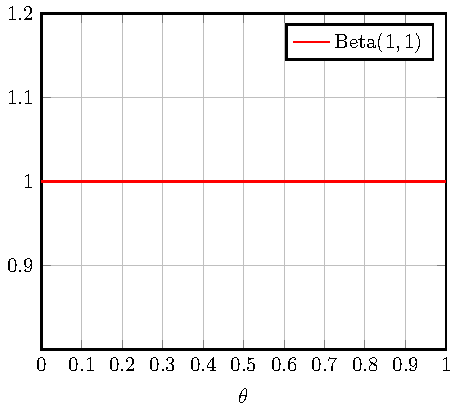
\includegraphics{Figures/Beta_1_1.pdf}
\end{minipage}
\begin{minipage}{0.5\textwidth}
  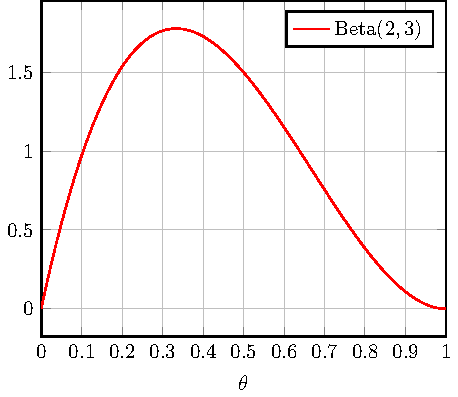
\includegraphics{Figures/Beta_2_3.pdf}
\end{minipage}
\begin{minipage}{0.5\textwidth}
  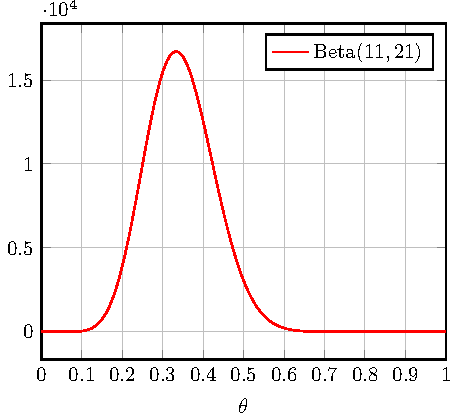
\includegraphics{Figures/Beta_11_21.pdf}
\end{minipage}
\begin{minipage}{0.5\textwidth}
  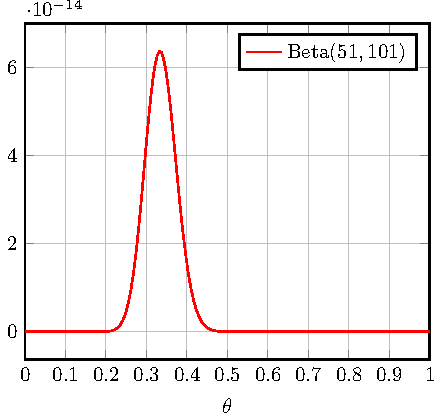
\includegraphics{Figures/Beta_51_101.pdf}
\end{minipage}

The above shows that we can perform estimation based on the number of experiments, which will result in a different PDF. With more data in hand, the accuracy of the data is higher. However, they share a common feature: the value at which the PDF or PMF reaches its maximum is 
\[
  \text{mode}[\theta] = \dfrac{\alpha - 1}{\alpha - 1 + \beta - 1} \quad \text{when}\ \alpha, \beta > 1
\] 

\begin{minipage}{0.5\textwidth}
  Also, we can treat the different parameters as a change in belief. For example, if Beta(2, 3) is our prior, and we readjust our belief based on observations, we then obtain Beta(21, 11). This shows that the area below the original mode \(\frac{1}{3}\) decreases, making it less probable. 

  The last thing to note is that hyperparameter, in the coin flip case, \(h, t\), don’t matter if we observe a large number of data samples, meaning the posterior mainly depends on the observed data. However, if the prior contains a large dataset or the size of the observed data is small, then the prior plays an important role in the posterior. 
\end{minipage}
\begin{minipage}{0.5\textwidth}
  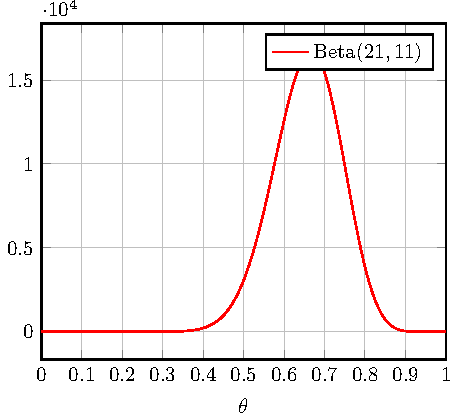
\includegraphics{Figures/Beta_21_11.pdf}
\end{minipage}

\subsection{Conjugate Prior for Poisson}
\begin{definition}
  Suppose \(X_1, \cdots, X_n\) form a random sample from Poisson distribution with an unknown mean \(\Theta > 0\). If the prior distribution \(f_{\Theta}(\theta)\) is the Gamma distribution \(\text{Gamma}(\alpha, \beta)\ (\alpha, \beta >0)\), then the posterior distribution \(f_{\Theta \vert X} (\theta \vert x)\) given \(\{X_i = x_i\}_{i=1} ^n\) is the Gamma distribution \(\text{Gamma}(\alpha + \sum_{i = 1}^n x_i, \beta + n)\). 
\end{definition}

Here we introduce another random variable that is often used as prior, Gamma random variable. It has the PDF as follows: 
\[
  f_{\Theta} (\theta) = \begin{dcases}
    \dfrac{\beta^{\alpha}}{\Gamma (\alpha)}\theta^{\alpha - 1} e^{-\beta\theta} &\text{ for } \theta > 0 \\
    0 &\text{ for } \theta \leq 0 \\
  \end{dcases}, 
\]
where 
\[
  \Gamma (\alpha) = \int_{0}^{\infty} x^{\alpha - 1} e^{-x} dx = (\alpha - 1)!\ (\text{for positive integer}\ \alpha).
\]
Again, we have the Gamma random variable as the denominator because the integral needs to be equal to 1.

\begin{eg}
  At an Apple Store, the number of iPhones sold per day is modeled as a Poisson distribution with unknown mean \(\Theta\). Suppose the prior distribution of \(\Theta\) is Gamma(3, 2). Let \(X\) be the number of iPhones sold in a specific day. If \(X = 3\) is observed, what is the updated distribution of \(\theta\)? 
  
  \textbf{Solution:} 
  Here we have 
  \[
    X \sim \text{Poisson}(\Theta) = \begin{dcases}
      \dfrac{e^{-\theta}\theta^x}{x!} &\text{ for } x = 0, 1, 2 \dots\\
      0  &\text{ otherwise} \\ 
    \end{dcases};
  \]
  \[
    \Theta \sim \text{Gamma}(\alpha, \beta) = \begin{dcases}
      \dfrac{\beta^{\alpha}}{\Gamma (\alpha)}\theta^{\alpha - 1} e^{-\beta\theta} &\text{ for } \theta > 0 \\
      0 &\text{ for } \theta \leq 0 \\
    \end{dcases}.
  \]
  Since we have observed \(X = 3\), 
  \[
    f_{\Theta \vert X} (\theta \vert 3) \propto f_{\Theta} (\theta) f_{X \vert \Theta} (3 \vert \theta)
  \]
  where
  \[
    f_{\Theta} (\theta) = \text{Gamma}(3, 2) = \dfrac{2^3}{2!}\theta^{3-1}e^{-2\theta}, f_{X \vert \Theta} (3 \vert \theta) = \text{Poisson}(\theta) = \dfrac{e^{-\theta}\theta^3}{3!}.
  \]
  Then we have
  \[
    f_{\Theta \vert X} (\theta \vert 3) \propto f_{\Theta} (\theta) f_{X \vert \Theta} (3 \vert \theta) = \dfrac{2^2}{3!} \theta^5 e^{-3\theta} \propto \theta^5 e^{-3\theta}
  \]
  \[
    f_{\Theta \vert X} (\theta \vert 3) = \dfrac{\theta^{6-1} e^{-3\theta}}{Z},\quad Z = \int_{0}^{\infty} \theta^{6-1} e^{-3\theta} d \theta = \dfrac{\Gamma(6)}{3^6}
  \]
  Finally, we have the posterior
  \[
    f_{\Theta \vert X} (\theta \vert 3) = \text{Gamma}(6, 3). 
  \]
\end{eg}

Above is the same as taking \(\alpha = 3, \beta = 2, n = 1 \text{ and } x = 3\), then we have \(\alpha + x = 6\), \(\beta + n = 3\). This directly gives us Gamma(6, 3). 

\subsection{Conjugate Prior for Exponential}
\begin{definition}
  Suppose \(X_1, \cdots, X_n\) form a random sample from Exponential distribution with an unknown parameter \(\theta > 0\). If the prior distribution \(f_{\Theta}(\theta)\) is the Gamma distribution \(\text{Gamma}(\alpha, \beta)\\ (\alpha, \beta > 0)\), then the posterior distribution \(f_{\Theta \vert X} (\theta \vert x)\) given \(\{X_i = x_i\}_{i=1} ^n\) is the Gamma distribution \(\text{Gamma}(\alpha + n, \beta + \sum_{i = 1}^n x_i)\). 
\end{definition}

In the case of Exponential prior, we have \(\alpha =\) no. of trials + 1, \(\beta =\) sum of data \(+\) prior. 

\begin{eg}
  If the number of iPhones sold per hour follows a Poisson distribution with unknown mean \(\Theta\), then the time between two successive iPhones sold follow an exponential distribution with parameter \(\Theta\). Suppose the prior distribution of \(\Theta\) is Gamma(1, 2). Let \(X\) be the time interval (in hour) between successive iPhones sold.

  Assume that we have \(X_1 = 1.5, X_2 = 2, X_3 = 2.5\). 

  \textbf{Solution:} 
  Here we have 
  \[
    X \sim \text{Exponential}(\Theta) = \begin{dcases}
      \theta e^{-\theta x} &\text{ for } x \geq 0 \\
      0  &\text{ for } x < 0 \\ 
    \end{dcases};
  \]
  \[
    \Theta \sim \text{Gamma}(1, 2). 
  \]
  Since we have observed \(X_1, X_2, X_3\), 
  \[
    f_{\Theta \vert X_1, X_2, X_3} (\theta \vert 1.5, 2, 2.5) \propto f_{\Theta} (\theta) f_{X_1, X_2, X_3 \vert \Theta} (1.5, 2, 2.5 \vert \theta)
  \]
  where
  \[
    f_{\Theta} (\theta) = \text{Gamma}(1, 2) = \dfrac{2^1}{1!}\theta^{1-1}e^{-2\theta}, f_{X_1, X_2, X_3 \vert \Theta} (1.5, 2, 2.5 \vert \theta) = (\theta e^{-1.5\theta}) (\theta e^{-2\theta}) (\theta e^{-2.5\theta}). 
  \]
  Then we have
  \[
    f_{\Theta \vert X_1, X_2, X_3} (\theta \vert 1.5, 2, 2.5) \propto f_{\Theta} (\theta) f_{X_1, X_2, X_3 \vert \Theta} (1.5, 2, 2.5 \vert \theta) = 2\theta^3 e^{-(2 + 6)\theta} \propto \theta^3 e^{-(2 + 6)\theta}
  \]
  \[
    f_{\Theta \vert X} (\theta \vert 3) = \dfrac{\theta^3 e^{-(2 + 6)\theta}}{Z},\quad Z = \int_{0}^{\infty} \theta^3 e^{-(2 + 6)\theta} d \theta = \dfrac{\Gamma(4)}{8^4}
  \]
  Finally, we have the posterior
  \[
    f_{\Theta \vert X} (\theta \vert 3) = \text{Gamma}(4, 8). 
  \]
\end{eg}

Above is the same as taking \(\alpha = 1, \beta = 2, n = 3, x_1 = 1.5, x_2 = 2 \text{ and } x_3 = 2.5\), then we have \(\alpha + n = \text{no. of trials} + 1 = 3 + 1= 4\), \(\beta + n = \text{sum of trials} + \text{prior} = 6 + 2 = 8\). This directly gives us Gamma(4, 8). 

\subsection{Conjugate Prior for Normal Distribution}
\begin{definition}
  Suppose \(X_1, \cdots, X_n\) form a random sample from a normal distribution with an unknown mean \(\mu\) and a known variance \(\sigma^2 > 0\). If the prior distribution \(f_{\Theta}(\mu)\) is the normal distribution \(\mathcal{N} (\mu, \sigma_0^2)\), then the posterior distribution \(f_{\Theta \vert X} (\mu \vert x)\) given \(\{X_i = x_i\}_{i=1} ^n\) is the normal distribution \(\mathcal{N}(\mu^{\prime}, \sigma^{\prime2})\), where 
  \[
    \mu^{\prime} = \dfrac{\sigma^2\mu_0 + \sigma_0^2 \sum_{i = 1}^n x_i}{\sigma^2 + n\sigma_0^2} \quad\quad \sigma^{\prime2} = \dfrac{\sigma^2\sigma_o^2}{\sigma^2 + n\sigma_o^2}
  \] 
\end{definition}

\begin{definition}[A more general case]
  Suppose \(X_1, \cdots, X_n\) form a random sample from a normal distribution with a common unknown mean \(\theta\) and the known variance \(\sigma_i^2 > 0\). If the prior distribution \(f_{\Theta}(\theta)\) is the normal distribution \(\mathcal{N} (\mu_0, \sigma_0^2)\), then the posterior distribution \(f_{\Theta \vert X} (\theta \vert x)\) given that \(\{X_i = x_i\}_{i=1} ^n\) is the normal distribution \(\mathcal{N}(\mu, \sigma^2)\), where 
  \[
    \dfrac{\mu}{\sigma^2} = \dfrac{\mu_0}{\sigma_0^2} + \dfrac{x_1}{\sigma_1^2} + \cdots + \dfrac{x_n}{\sigma_n^2} \quad\quad \dfrac{1}{\sigma^2} = \dfrac{1}{\sigma_0^2} + \dfrac{1}{\sigma_1^2} + \cdots + \dfrac{1}{\sigma_n^2}
  \] 
\end{definition}

Here we need to consider a special case when both \(\sigma_0^2\) and \(\sigma^2\) are equal to 1, then we have 
\[
  \mu^{\prime} = \dfrac{\mu_0 + \sum_{i = 1}^n x_i}{1 + n} \quad\quad \sigma^{\prime2} = \dfrac{1}{1 + n}
\]

\begin{eg}
  An \(\mathcal{N}(\Theta, 1)\) random variable takes value 3.97. \(\Theta\) follows a standard normal. What is the posterior of \(\Theta\)?
  
  \textbf{Solution:} 
  Here we have the PDF of \(\mathcal{N} (\mu, \sigma^2)\) 
  \[
    f_X(x) = \dfrac{1}{\sigma \sqrt{2\pi}} e^{-\frac{1}{2}\frac{(x - \mu)^2}{\sigma^2}}
  \]
  Given that the prior = \(\Theta \sim \mathcal{N}(0, 1)\), posterior = \(f_{\Theta \vert X}(\theta \vert x) \propto f_{\Theta} (\theta) f_{X \vert \Theta} (x \vert \theta)\), we have
  \[
    f_{\Theta} (\theta) = \dfrac{1}{\sqrt{2\pi}}e^{-\frac{1}{2}\theta^2} \quad\quad f_{X \vert \Theta} (x \vert \theta) = \dfrac{1}{\sqrt{2\pi}}e^{-\frac{1}{2}(x - \theta)^2}
  \]
  \[
  \begin{aligned}
    f_{\Theta \vert X}(\theta \vert x) \propto f_{\Theta} (\theta) f_{X \vert \Theta} (x \vert \theta) &= \dfrac{1}{\sqrt{2\pi}}e^{-\frac{1}{2}\theta^2} \times \dfrac{1}{\sqrt{2\pi}}e^{-\frac{1}{2}(x - \theta)^2} \\
    &\propto e^{-\frac{1}{2}\theta^2} \times e^{-\frac{1}{2}(x - \theta)^2} \\
    &= e^{-\frac{1}{2}\theta^2 -\frac{1}{2}(x - \theta)^2} \\
    &= e^{-(\sqrt{2}\theta - \frac{1}{\sqrt{2}}x)^2} \underbrace{e^{-\frac{x^2}{4}}}_{\text{constant term}} \\ 
    &\propto e^{-(\sqrt{2}\theta - \frac{1}{\sqrt{2}}x)^2} \\ 
    &= e^{-\frac{1}{2}\frac{(\theta - \frac{x}{2})^2}{(\frac{1}{\sqrt{2}})^2}} \\ 
  \end{aligned}
  \]
  Then we have
  \[
    \mu = \dfrac{x}{2} = \dfrac{3.97}{2} = 1.985 \quad\quad \sigma^2 = (\dfrac{1}{\sqrt{2}})^2 = \dfrac{1}{2}
  \]
  Finally, we have the posterior
  \[
    f_{\Theta \vert X} (\theta \vert 3) = \mathcal{N} (1.985, \dfrac{1}{2})
  \]
\end{eg}

Above is the same as taking \(\mu_0 = 0, x_1 = 3.97, \sigma_0 = 1 \text{ and } \sigma_1 = 1\), then we have 
\[
  \dfrac{1}{\sigma^2} = \dfrac{1}{1} + \dfrac{1}{1} \Longrightarrow \sigma = \dfrac{1}{\sqrt{2}} \quad\quad \dfrac{\mu}{\frac{1}{2}} = \dfrac{0}{1} + \dfrac{3.97}{1} \Longrightarrow \mu = 1.985, 
\]
which directly gives us \(\mathcal{N} (1.985, \dfrac{1}{2})\). 

When \(\sigma_0 = \sigma_1 = \cdots = 1\), we can find \(\sigma\) and \(\mu\) by:
\[
  \sigma = \dfrac{1}{\sqrt{n + 1}}, \quad \mu = \dfrac{x_0 + x_1 + \cdots + x_n}{n + 1}
\] 

\begin{eg}
  Three independent \(\mathcal{N}(\Theta, 1)\) random variables take values 3.97, 4.09, 3.11. What is \(\Theta\)? 
  
  \textbf{Solution:} 
  Here we assume the priors are \(\Theta \sim \mathcal{N} (0, 1)\), and from observation we have \(x_1 = 3.97, x_2 = 4.09, x_3 = 3.11\). 

  Then, for the posterior, we have 
  \[
    f_{\Theta \vert X_1, X_2, X_3} (\theta \vert x_1, x_2, x_3) \sim \mathcal{N} \left(\dfrac{0 + 3.97 + 4.09 + 3.11}{1 + 3}, \left(\dfrac{1}{\sqrt{1 + 3}}\right)^2\right) \approx \mathcal{N} (2.79, \dfrac{1}{4})
  \]
\end{eg}

% L02 finished
% END OF DOCUMENT